\documentclass[10pt,showpacs,preprintnumbers,footinbib,amsmath,amssymb,aps,prl,twocolumn,groupedaddress,superscriptaddress,showkeys]{revtex4-1}
\usepackage{graphicx}
\usepackage{dcolumn}
\usepackage{bm}
\usepackage[colorlinks=true,urlcolor=blue,citecolor=blue]{hyperref}
\usepackage{color}


\begin{document}

\title{First-principles calculations for coefficients of the isobaric
mass multiplet equation in the fp shell}


\author{W.~E.~Ormand}
\affiliation{Lawrence Livermore National Laboratory, Livermore, CA 94551, USA}
\author{B.~A.~Brown} 
\affiliation{Department of Physics and Astronomy and National Superconducting Cyclotron Laboratory,
Michigan State University, East Lansing, MI 48824-1321, USA}
\author{M.~Hjorth-Jensen}
\affiliation{Department of Physics and Astronomy and National Superconducting Cyclotron Laboratory,
Michigan State University, East Lansing, MI 48824-1321, USA}
\affiliation{Department of Physics, University of Oslo, N-0316, Oslo, Norway}

\begin{abstract}
We present the first calculations for the $c$-coefficients of the isobaric
mass multiplet equation (IMME)
for nuclei from $A=42$ to $A=54$ based on input from several realistic nucleon-nucleon interactions.
We show that there is clear dependence on the short-ranged charge-symmetry
breaking (CSB) part of the strong interaction. There is a significant
variation in the CSB part between the commonly
used CD-Bonn, N$^3$LO and Argonne V18 nucleon-nucleon
interactions. All of them give a CSB contribution that is too large when 
compared to experiment.
\end{abstract}

\pacs{21.30.Fe, 21.60.Cs, 21.60.De, 27.40.+z}


\maketitle

Isospin is a powerful spectroscopic tool in nuclear physics that can
be used to label and characterize states not only in a specific
nucleus, but also corresponding states in an analog nucleus. Isospin,
denoted by $T$, is an additive quantity similar to the intrinsic spin
of the proton and neutron. The charge, $Q$, of the particle is defined
by the $z$-component via $Q=\frac{1}{2} + T_z$. Thus, for a nucleus
with $Z$ protons and $N$ neutrons, the $z$-component is $T_z=(Z-N)/2$,
and a nucleus may have isospin states with $T \ge T_z$, Isospin
symmetry is broken by components in the nuclear Hamiltonian that treat
protons and neutrons differently. The most obvious, and significant,
component is the Coulomb interaction acting only between protons due
to their electric charge. There are, however, weaker isospin-symmetry
breaking components in the nucleon-nucleon interaction itself caused
by differences in the masses of up and down quarks and their intrinsic
electric charges, which is reflected in the slightly different masses
exhibited by neutrons and protons \cite{miller2006} and the slightly
different strong-interaction scattering lengths observed in the
proton-proton ($pp$), neutron-neutron ($nn$), and the $T=1$
proton-neutron ($pn$) channels.

Important signatures of isospin-symmetry breaking interactions are
differences in the binding energy of nuclei within the same isospin
multiplet with fixed nucleon number $A$. These mass splittings, or
Coulomb-displacement energies offer a sensitive probe of the
properties of isospin-symmetry breaking in nuclei. The three $T=1$
nucleon-nucleon channels can be decomposed into three isospin
components: isoscalar (rank 0), isovector (rank 1), and isotensor
(rank 2), defined in terms of the $pp$, $nn$, and $pn$ interactions
via
\begin{align}
\label{e:1}
v^{(0)} & =  \frac{1}{3} (v_{pp} + v_{nn} + v_{pn}) \\
\label{e:2}
v^{(1)} & =  (v_{pp} - v_{nn}) \\
\label{e:3}
v^{(2)} & =  v_{pn} - \frac{1}{2}(v_{pp} + v_{nn}).
\end{align}
With these three components, the masses for a set of states within a multiplet with isospin $T$ may be described by the isobaric mass multiplet equation (IMME)
\begin{equation}
M (T_z) = a + bT_z + cT_z^2,
\end{equation}
where the coefficients $a$, $b$, and $c$ are dependent on the
isoscalar, isovector, and isotensor components of the nuclear
Hamiltonian, respectively. The linear and quadratic dependence on
$T_z$ is due to the application of the Wigner-Ekhart theorem and the
appropriate Clebsch-Gordon coefficients arising for the isovector and
isotensor components of the Hamiltonian, respectively.

In this letter, we compute Coulomb-displacement energies as a function
of excitation for nuclei in the mass range $42 \le A \le 54$ using the
isospin-symmetry breaking interactions derived from realistic
nucleon-nucleon interactions. Here, we focus on the effects of the
isotensor component as exhibited in the $c$-coefficient of the IMME.


We performed a series of shell-model calculations using the program
BIGSTICK to compute the $c$-coefficients of the IMME for $1p0f$-shell
nuclei with $ 42 \le $ A $ \le 54$. The pertinent effective
interactions for the degrees of freedom of the $1p0f$ shell were
derived using many-body perturbation theory, see for example
Ref.~\cite{mhj1995}. The two-body matrix elements where computed in
two steps, first by renormalizing the nuclear two-body interactions
using both a $G$-matrix approach and the so-called V$_{lowk}$
method. For the nuclear interactions, we employed the realistic
N$^3$LO \cite{entem2003}, AV18 \cite{argonne1995} and CD-Bonn
\cite{cdbonn2001} nucleon-nucleon interactions. These interaction
models allow for the breaking of isospin symmetry and charge symmetry
and include the isotensor and isovector components of the strong
interaction.  The reader should note that the AV18 interaction model includes electromagnetic corrections
and the full model is used when renormalizing the short-range part of the force. 
This may lead to slightly different Coulomb interactions in a finite nucleus. 
The renormalized nucleon-nucleon interactions were
computed using a harmonic oscillator basis with an oscillator energy
$\hbar\omega =10.5$ MeV with an effective Hilbert space defined by the
first twelve oscillator shells. The $G$-matrix and V$_{lowk}$ interactions were
obtained with a cut-off parameter of $\Lambda$ = 2.1 fm$^{-1}$.  For
the N$^3$LO and the CD-Bonn interactions, the Coulomb interaction was
added after the renormalization process.  The second step consisted in
obtaining an effective interaction tailored to a small shell-model
space. This was achieved using many-body perturbation theory up to
third order in the renormalized nucleon-nucleon interactions,
including so-called folded diagrams \cite{mhj1995}. All codes used to
generate these interactions are publicly available~\cite{mhjgit}.  The
renormalization was performed with and without the Coulomb
interaction, and the Coulomb two-body matrix elements were obtained
from the difference between these proton-proton ($pp$) matrix
elements. The renormalized interaction computed without Coulomb was
then decomposed into the three isospin components: isoscalar (rank 0),
isovector (rank 1), and isotensor (rank 2), as defined in
Eqs.~(\ref{e:1})-(\ref{e:3}).

The $c$-coefficients of the IMME were obtained utilizing first-order
perturbation theory. The base for each calculation was the eigenstate,
$E_{0}$ for each member of the $T=1$ triplet, $ \vert T_{z} \rangle$,
obtained using the isoscalar GX1A Hamiltonian~\cite{ref:GX1A}. The
GX1A interaction was used instead of the $v^{(0)}$ interaction
obtained from the realistic interaction described above because of
well-known extensions that must be included to properly capture the
behavior of higher-order components and the three-body interaction in
the traditional configuration-interaction shell model for atomic
nuclei, see for example Refs.~\cite{zuker2003,ekstrom2015}. The expectation value of the Coulomb,
isovector, and isotensor interactions are then computed to give the
full energy for each state,
\[
E(T_{z}) = E_{0} + \langle T_{z} \vert   v^{{\rm Coul}} + v^{(1)} + v^{(2)}\vert T_{z} \rangle
\]
and the c-coefficient is then computed from
\[
c = [E(T_{z} =1) - 2E(T_{z} =0) + E(T_{z} =-1)]/2.
\]
The $A$-dependence was properly accounted for by scaling the Coulomb
matrix elements by $ \sqrt{\hbar\Omega(A)/10.5} $, while the isovector
and isotensor interactions were assumed to have the same
$A$-dependence as the GX1A interaction. For each $A$-value,
$\hbar\Omega(A)$ was determined by reproducing the {\it rms} radius
obtained from a Hartee-Fock calculation for $42 \le A\le 54$ nuclei
using the SkX Skyrme interaction \cite{ref:SkX}.

Figure 1 shows the results CD-Bonn to first, second and third order in many-body perturbation theory.
The contributions are divided into Coulomb (full lines) and CSB
(dashed lines). The $J$-dependence of these two contributions is very
different. The long-range Coulomb has a relatively flat $J$-dependence
with only a small rise at $J=0$. The CSB contribution at $A=42$ shows
a peak at $J=0$ with a sharp drop towards $J=2$, which is
characteristic of a short-ranged interaction.  
This pattern is observed if one employs a simple $\delta$-function interaction model.

For $A=42$, $J=6$ is
the maximum angular momentum (for $T=1$) in the $1p0f$ model space.
For higher values of $A$, this sharp drop at $ J=2 $ is replaced by a
linear drop to $J=6$ due to configuration mixing.  We note that for
$J=8$ and $10$, the effect of charge-symmetry breaking is small. The
experimental data is taken from the compilation \cite{2013la}, except
for $A=46$, where we use the results from Fig.~2 of \cite{2001ga}.

Both Coulomb and CSB have a small increase at $J=12$.
The reason for this is that
protons with $J=6$ and neutrons with $J=6$
are maximally aligned, resulting in an enhancement of the
overlapping proton and neutron density distributions.

\begin{figure}
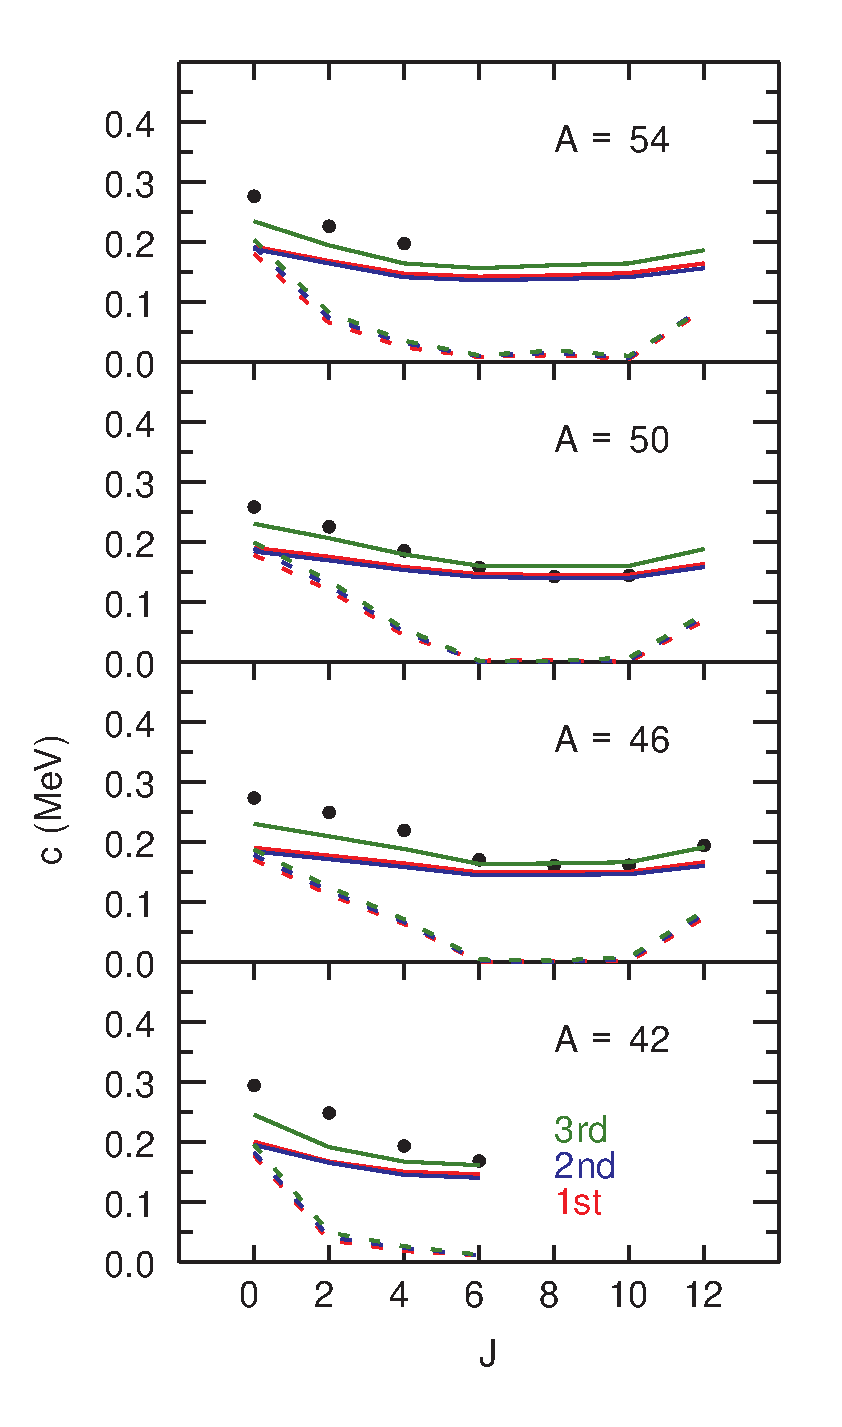
\includegraphics[scale=0.35]{ccd.eps}
\caption{(color online) Results for the CD-Bonn potential
in 1$^{\rm st}$, up to 2$^{\rm nd}$ and up to 3$^{\rm rd}$ order.
The black circles
are the experimental data. The solid lines show the Coulomb
contribution, and the dashed lines show the CSB contribution.}
\end{figure}
\begin{figure}
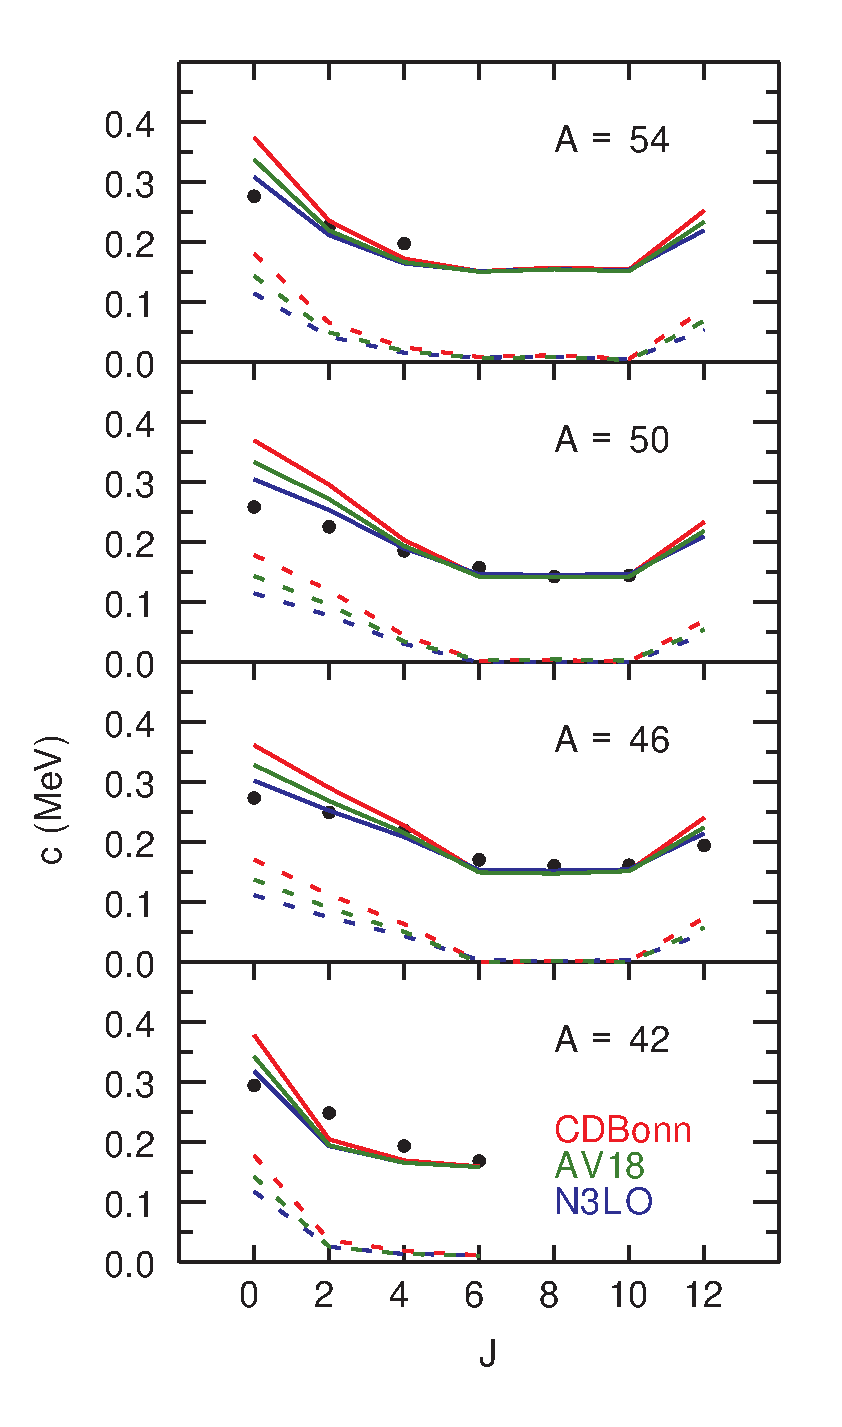
\includegraphics[scale=0.35]{c1.eps}
\caption{(color online) 1$^{\rm st}$ order calculations compared to
experiment. The black circles
are the experimental data. The solid lines show the sum of Coulomb and
CSB
contributions. The dashed lines show only the CSB contribution.}
\end{figure}
\begin{figure}
\includegraphics[scale=0.35]{c3.eps}
\caption{(color online) Calculations up to 3$^{\rm rd}$ order compared to
experiment. See caption to Fig 2.}
\end{figure}
\begin{figure}
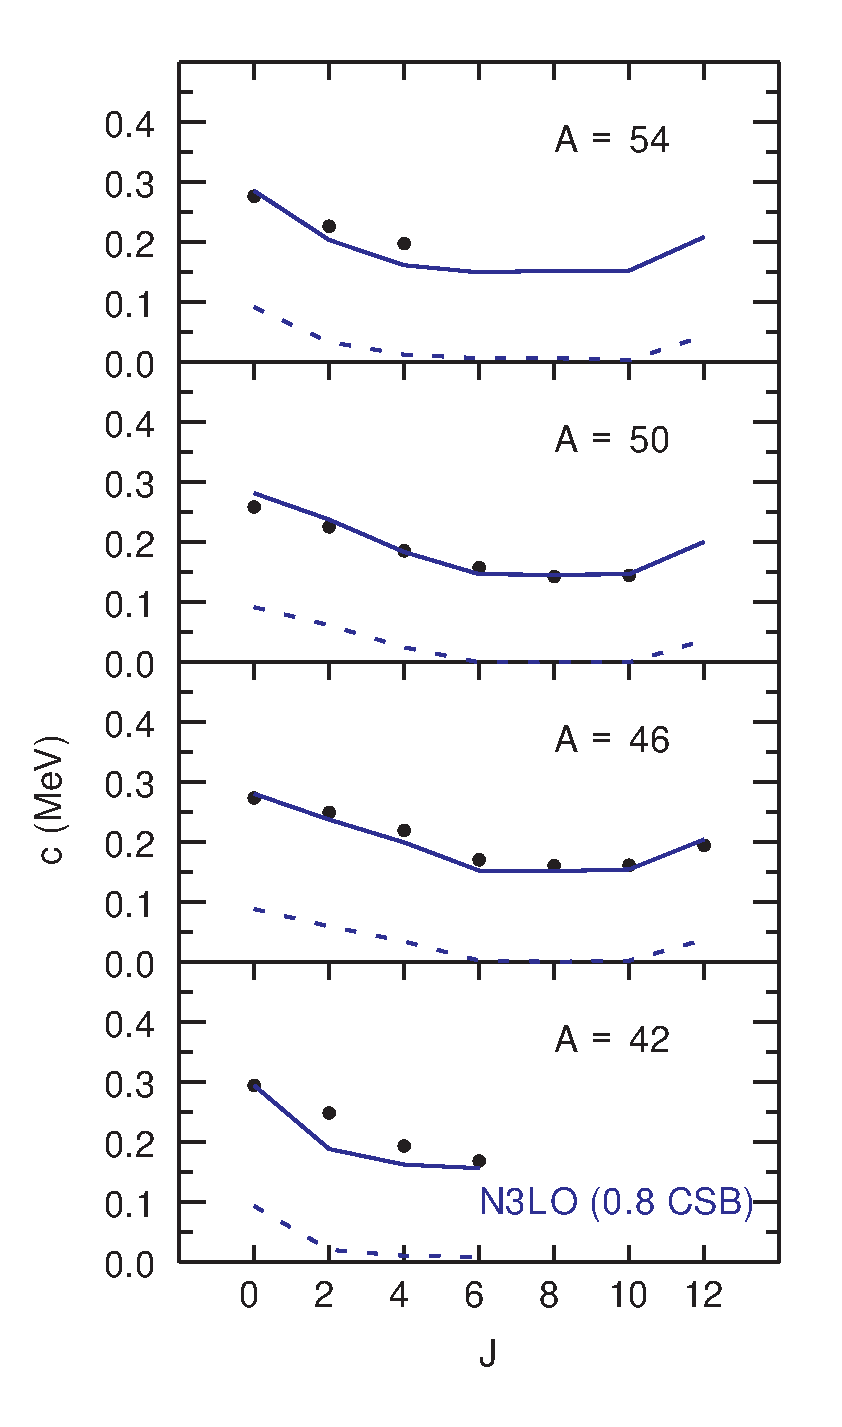
\includegraphics[scale=0.35]{c1e.eps}
\caption{(color online) 1$^{\rm st}$ order calculations for N$^3$LO
with the CSB part multiplied by 0.8 and compared to
experiment. See caption to Fig 2.}
\end{figure}



The CSB contribution turns out to be almost order independent, while
the Coulomb contribution is almost the same to first and
second order in many-body perturbation theory, but increases by 10-20\% to third
order. This suggests that the CSB interaction is substantially
short-ranged in nature, and the $G$-matrix and $V_{lowk}$ treatment
may be sufficient. A simple analysis of all $J=0$ two-body matrix elements, using
Eqs.~(\ref{e:1})-(\ref{e:2}), shows that for the core-polarization contribution to second order, the 
correction to $c$ is about ten times smaller than that for $a$. This applies to most two-body matrix elements 
that define Eqs.~(\ref{e:1})-(\ref{e:2}).

It is remarkable that the experimental data are in
rather good agreement with the third order Coulomb result,
where there seems to be no need for CSB even though this component is
well known to be important in nucleon-nucleon ($NN$) scattering data that is incorporated
into the potential models.

Figure 2 shows the results for the three potential models 
to first order in interaction.  This shows that the CSB contribution is model
dependent.  There could be a few reasons for this. While the $NN$
interactions are all fit to scattering data and reproduce the
proton-neutron scattering length equally well, there could be
differences in the underlying treatment of the CSB components.  In
addition, while AV18 is a purely local potential, both N$^3$LO and
CD-Bonn are non-local, albeit in different ways. Finally, the
short-range correlation effects taken into account in the $G$-matrix and V$_{lowk}$
renormalizations could have different effects on this small component
of the $NN$ interactions, which may be corrected when induced
three-nucleon terms are included.  We note that the results obtained
with N$^3$LO are in best agreement with experiment, although all three
interactions over predict the $c$-coefficients. This in its own self
might be a signature of charge-symmetry breaking in the initial three
nucleon interaction.

Figure 3 shows the results for the three potentials to third order.

Our work guides future investigations in directions.  For better first
principles calculations, one should understand the origin of the
different CSB contributions from these three realistic potentials.  In
particular, in the spirit of using nuclear data to constrain the $NN$
and three-nucleon ($3N$) interactions (in addition to $NN$ scattering data) one should use
the $c$-coefficient as a constraint on the CSB part. From a practical
point of view, we start with the fact that first-order Coulomb
plus CSB is already close to the data.  We can make it almost perfect
by taking the first-order Coulomb contribution and add 80\% of the N$^3$LO
CSB part. This is shown in Fig.~4.  The largest deviation from
experiment comes for $ J=2 $ at $A=42$.  However, $ A=42 $ is just at
the beginning of the $ 1p0f $ model space and it is well know that
admixtures from core excitations from the $0s-1d $ shell are very
important especially for $J=0$ and $J=2$.  For example, the 2$^{ + }$
to 0$^{ + }$ B(E2) value for $^{42}$Ca is about ten times larger in
experiment than compared to theory. The experimental fall off from $J=0 $ 
to $ J=6 $ in $A=42$ looks like calculation for $A=46$. The
theoretical wave functions for A=42 are dominated by $ (f_{7/2})^{2} $
configurations and the wave functions for $ A=54 $ are dominated by $(f_{7/2})^{-2} $ 
configurations. These two configuration have the same
spectra (except for a small mass dependence).  Compared to $ A=42 $
the $ J $ dependence observed for $ A=54 $ is closer than expected for
these pure configurations.

In conclusion, we have presented the first calculations for the
$c$-coefficients of the IMME for nuclei from $A=42$ to $A=54$, based
on input from several realistic nucleon-nucleon interactions and their
pertinent shell-model effective interactions. The CSB contribution is
almost independent of the order of renormalization in many-body
perturbation theory, suggesting that the charge-symmetry breaking part
of the interaction is to a large extent of a short-range nature.  In
effective field theory this may point to two-pion or higher-pion
excitations that probe the short range nature of the CSB interaction.
Whether these conclusions remain when three-body interactions
are included, given the short-range nature of the CSB part of the
interactions, remains to be seen.



BAB acknowledges U.S. NSF Grant No. PHY-1404442. MHJ acknowledges
U.S. NSF Grant No. PHY-1404159 and the Research Council of Norway
under contract ISP-Fysikk/216699. WEO acknowledges support from the
U.S. Department of Energy, Office of Science, Office of Nuclear
Physics, under Field Work Proposal No. SCW0498. This work was
performed under the auspices of the U.S. Department of Energy by
Lawrence Livermore National Laboratory under Contract
DE-AC52-07NA27344.  Computing support for this work came from the
Lawrence Livermore National Laboratory (LLNL) institutional Computing
Grand Challenge program.

\begin{thebibliography}{99}
\bibitem{miller2006} G.~A.~Miller, A.~K.~Opper, and E.~J.~Stephenson, Annu.~Rev.~Nucl.~Sci.~{\bf 56}, 253 (2006).
\bibitem{2013la} Y.~H.~Lam, B.~Blank, N.~A.~Smirnova, J.~B.~Bueb, and M.~S.~Antony, At.~Data and Nucl.~Data Tables {\bf 90}, 680 (2013). 
\bibitem{2001ga} P.~E.~Garrett {\em et al.}, Phys.~Rev.~Lett.~{\bf 87}, 132502 (2001). 
\bibitem{mhj1995} M.~Hjorth-Jensen, E.~Osnes, and T.~.T.~.S.~Kuo, Phys.~Rep.~{\bf 261}, 125 (1995).
\bibitem{entem2003} D.~R.~Entem and R.~Machleidt, Phys.~Rev.~C {\bf 68}, 041001(R) (2003).
\bibitem{argonne1995} R.~B.~Wiringa, V.~G.~J.~Stoks, and R.~Schiavilla, Phys.~Rev.~C {\bf 51}, 38 (1995).
\bibitem{cdbonn2001} R.~Machleidt, Phys.~Rev.~C {\bf 63}, 024001 (2001).
\bibitem{mhjgit} All codes used to generate the effective interactions are available at \url{ https://github.com/ManyBodyPhysics/CENS}.
\bibitem{ref:GX1A} M.~Honma, T.~Otsuka, B.~.A.~Brown, and T.~Mizusaki, Phys. Rev. C {\bf 65}, 061301(R) 2002;
Euro. Phys. Jour. A {\bf 25 Suppl.} 1 499 (2005).
\bibitem{ref:SkX}B.~A.~Brown, Phys. Rev. C {\bf 58}, 220 (1998).
\bibitem{zuker2003} A.~P.~Zuker, Phys.~Rev.~Lett.~{\bf 90}, 042502 (2003).
\bibitem{ekstrom2015} A.~Ekstr\"om, G.~R.~Jansen, K.~A.~Wendt, G.~Hagen, T.~Papenbrock, B.~D.~Carlsson, C.~Forssen, M.~Hjorth-Jensen, P.~Navratil, and W.~Nazarewicz, Phys.~Rev.~C {\bf 91}, 051301(R) (2015).
\end{thebibliography}

\end{document}



